\documentclass[34pt]{beamer}
%\usetheme{default}
%\usetheme{Madrid}
%\usetheme{AnnArbor}
\usetheme{CambridgeUS}
%\usetheme{Copenhagen}
%\usetheme{Warsaw}
\usecolortheme{beaver}

\usepackage{color}
\usepackage{amsmath}
\usepackage{amssymb}
\usepackage{amsthm}
\usepackage{amscd}
\usepackage{eucal} % for \mathcal 

\usepackage{mathtools}% for using \mathclap,\smashoperator to reduce space after and before a sum.

\usepackage{amssymb,amsmath,bbm}
\usepackage{amscd}
\usepackage{graphicx}

\usepackage{tikz}
%\usepackage[french]{babel}
\usepackage[utf8]{inputenc}
\usepackage[all]{xy}


\usefonttheme[onlymath]{serif}

\usepackage{hyperref}
\hypersetup{
	colorlinks   = true,          %Colors links instead of ugly boxes
	urlcolor     = blue,          %Color for external hyperlinks
	linkcolor    = blue,          %Color of internal links
	citecolor   = red             %Color of citations
}



\setbeamertemplate{theorems}[numbered]

\title[Semester project]{Security analysis of Bluetooth Low Energy Over-The-Air firmware updates}
\author[Huy Hung LE]{Huy Hung LE\\[0.5cm]{\small Superviors:}\\ Aur\'elien Francillon\\Romain Cayre}
\institute{Eurecom}
\date{June 29, 2023}
% Remove the % from the previous line and change the date if you want a particular date to be displayed; otherwise, today's date is displayed by default.

\AtBeginSection[]  % The commands within the following {} will be executed at the start of each section.
{
	\begin{frame}[noframenumbering,plain] % Within each "frame" there will be one or more "slides."
		\frametitle{Presentation Outline} % This is the title of the outline.
		\tableofcontents[currentsection]  % This will display the table of contents and highlight the current section.
	\end{frame}
} % Do not include the preceding set of commands if you prefer not to have a recurring outline displayed during your presentation.



%%%%%%%%%%%%backup
%\makeatother
%\setbeamertemplate{footline}
%{
%	\leavevmode%
%	\hbox{%
%		\begin{beamercolorbox}[wd=.4\paperwidth,ht=2.25ex,dp=1ex,center]{author in head/foot}%
%			\usebeamerfont{author in head/foot}\insertshortauthor
%		\end{beamercolorbox}%
%		\begin{beamercolorbox}[wd=.6\paperwidth,ht=2.25ex,dp=1ex,center]{title in head/foot}%
%			\usebeamerfont{title in head/foot}\insertshorttitle\hspace*{3em}
%			\insertframenumber{} / \inserttotalframenumber\hspace*{1ex}
%	\end{beamercolorbox}}%
%	\vskip0pt%
%}
%\makeatletter
%
%\setbeamertemplate{navigation symbols}{}
%%%%%%%%%%%%%%%%%


%%%%%%%%%%%
\makeatother
\setbeamertemplate{footline}
{
	\leavevmode%
	\hbox{%
		\begin{beamercolorbox}[wd=1\paperwidth,ht=2.25ex,dp=7ex,right]{bgcolor}%
			\insertframenumber{} / \inserttotalframenumber\hspace*{20pt}
	\end{beamercolorbox}}%
	\vskip0pt%
}
\makeatletter

\setbeamertemplate{navigation symbols}{}
%%%%%%%%%%%%%%%%



%%%%%%%%%%%
\makeatother
\setbeamertemplate{headline}
{
	
}
\makeatletter

\setbeamertemplate{navigation symbols}{}
%%%%%%%%%%%%%%%%

\begin{document}
	
	\begin{frame}[noframenumbering,plain]
		\titlepage
	\end{frame}
	
	%\begin{frame} % Within each "frame" there will be one or more "slides."
	%	\frametitle{Presentation Outline} % This is the title of the outline.
	%	\tableofcontents[sectionstyle=show/show,subsectionstyle=show/show]  % This will display the table of contents and highlight the current section.
	%\end{frame}
	
	\begin{frame}
		%\frametitle{Plan of the talk}
		\tableofcontents
	\end{frame}
	
	
	\section{Device firmware updates}

	
	\begin{frame}
		\frametitle{Device firmware updates (DFU)}
		
		- DFU over-the-air is a process that allow to update firmware running on a device over BLE from a smartphone or a laptop
		
		\vspace{0.5cm}
		- Nordic Semiconductor provides a proprietary DFU process which implemented as a BLE Generic Attribute (GATT) Service
		
		\vspace{0.5cm}
		- nRF51 and nRF52 from Nordic Semiconductor are widely used in smartwatches, smartlocks
	
	\vspace{0.5cm}
		\pause- Goals
		\begin{itemize}
			\item Reverse engineer the DFU process
			\item Analysis the security of this process
		\end{itemize}
	\end{frame}

%	\begin{frame}
%		\frametitle{Doing DFU on Development Kit (DK)}
%		\begin{itemize}
%			\item Compiling files from nRF5 SDK (v9.0.0-v17.1.0)\\ \texttt{gcc-arm-none-eabi}
%			\item Flashing the complied files to the board\\
%			\texttt{nrfjprog}
%			\item Creating firmware packages\\
%			\texttt{nrfutil}
%			\item Doing the DFU
%			\texttt{nrfConnect} in Android
%		\end{itemize}
%	\end{frame}

	
	\section{Reverse engineer the DFU protocol }
	
	\subsection{Capture packages over the air}
	\begin{frame}
		\frametitle{Capture packages over the air}
		\begin{itemize}
			\item  Using Bluetooth HCI snoop log feature of Android phone
			\vspace{2cm}
			\pause\item Using another DK and Wireshark
		\end{itemize}

	\end{frame}
	\subsection{DFU protocol}
	\begin{frame}
		\frametitle{Results}
		\begin{columns}[T] % align columns
			\begin{column}{.48\textwidth}
				Open bootloader
				\rule{\linewidth}{4pt}
				
				1. Trigger the DFU process\\
				2. Start DFU process\\
				3. Send length of sd, bl, app\\
				4. Init DFU parameter\\
				5. Send init packet\\
				6. Init DFU parameter complete\\
				7. Set PRN value to 10\\
				8. Prepare to send firmware\\
				9. Send the firmware
			\end{column}%
			\hfill%
			\begin{column}{.48\textwidth}
				Secure bootloader
				\rule{\linewidth}{4pt}
				1. Trigger the DFU process\\
				2. Select Command Object\\
				3. Set PRN value to 0\\
				4. Create Command Object\\
				5. Send init package\\
				6. Calculate CRC\\
				7. Execute the sent file\\
				8. Set PRN value to 10\\
				9. Send the firmware
				(More complicated than open bootloader)
			\end{column}%
		\end{columns}
	\end{frame}
	\subsection{Python program}
	\begin{frame}
		\frametitle{Python program}
		\begin{itemize}
			\item Using Whad-client framework by Romain Cayre
			\vspace{1cm}
			\item Scan, connect, discovery services and characteristics
			\vspace{1cm}
			\item Search UUID in a database to find the corresponding name
			\vspace{1cm}
			\item With a firmware zip file, automatic unzip, read the data, process with the file then do the DFU process
		\end{itemize}

	\end{frame}
	\begin{frame}
		\frametitle{Screenshots - Open bootloader}
	\begin{figure}[H]
		\centering
		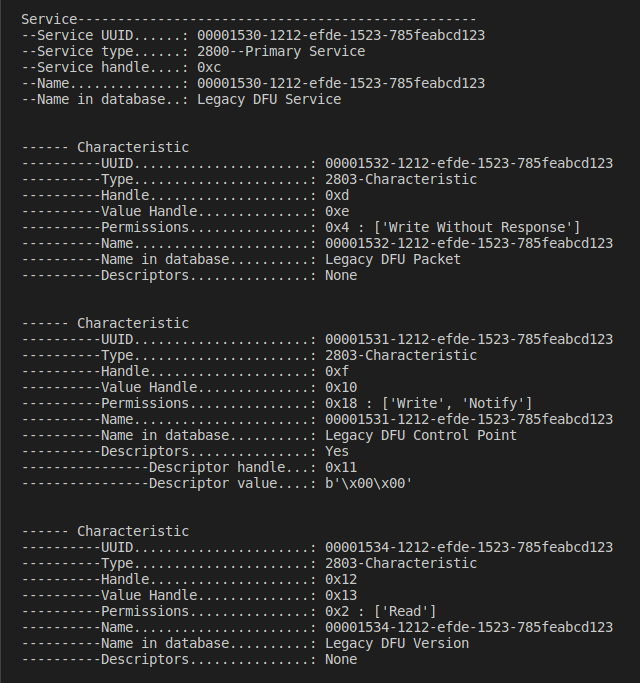
\includegraphics[width=0.64\linewidth]{../project_Report/images/gatt-open}
	\end{figure}
	\end{frame}	
	\begin{frame}
		\frametitle{Screenshots - Secure bootloader}
		\begin{figure}[H]
			\centering
			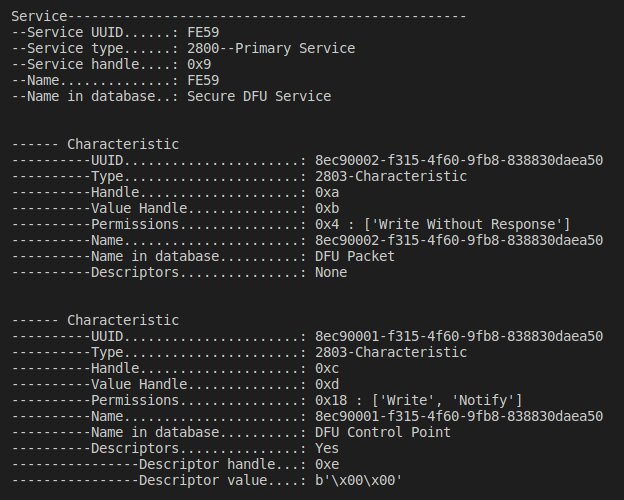
\includegraphics[width=0.80\linewidth]{../project_Report/images/gatt-secure}
		\end{figure}
	\end{frame}

\section{Reverse firmware packages}
\subsection{File manifest.json}
\begin{frame}
	\frametitle{File manifest.json}
		Open bootloader:
	\begin{figure}[H]
		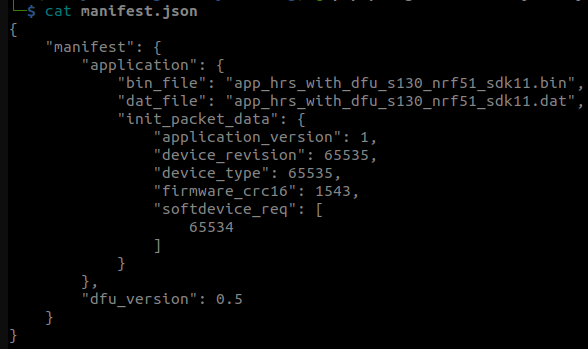
\includegraphics[width=0.6\linewidth]{../project_Report/images/manifest-open}
	\end{figure}
	Secure bootloader:
\begin{figure}[H]
	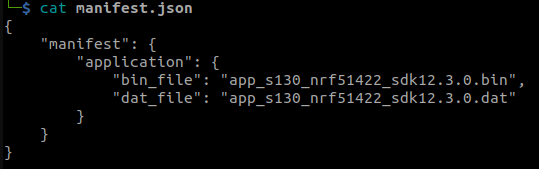
\includegraphics[width=0.6\linewidth]{../project_Report/images/manifest-secure}
\end{figure}

\end{frame}

\subsection{File .dat}
\begin{frame}
	\frametitle{File .dat}
	Open bootloader:
\begin{figure}[H]
	\centering
	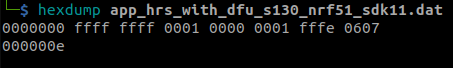
\includegraphics[width=0.9\linewidth]{../project_Report/images/dat-open}
\end{figure}
Secure bootloader:
\begin{figure}[H]
	\centering
	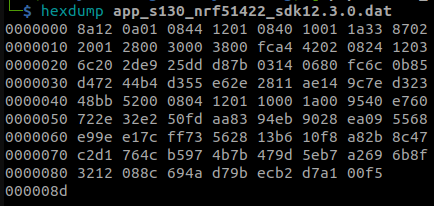
\includegraphics[width=0.9\linewidth]{../project_Report/images/dat-secure}
\end{figure}

\end{frame}
\begin{frame}
	\frametitle{File .dat - secure bootloader}
	
\begin{figure}[H]
	\centering
	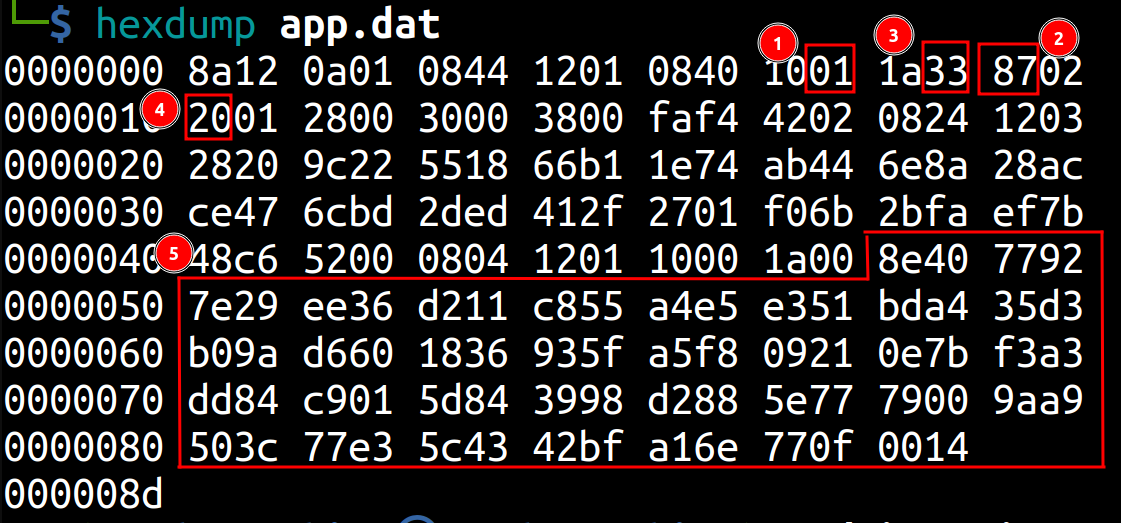
\includegraphics[width=0.7\linewidth]{../project_Report/images/reverse-dat-file-secure}
\end{figure}
\begin{center}
	1. application-version\\
2. sd-req\\
3+4. may related to hardware\\
5. signature of the hash	

\end{center}

\end{frame}

\begin{frame}
	\frametitle{File .dat - open bootloader}
	
\begin{figure}[H]
	\centering
	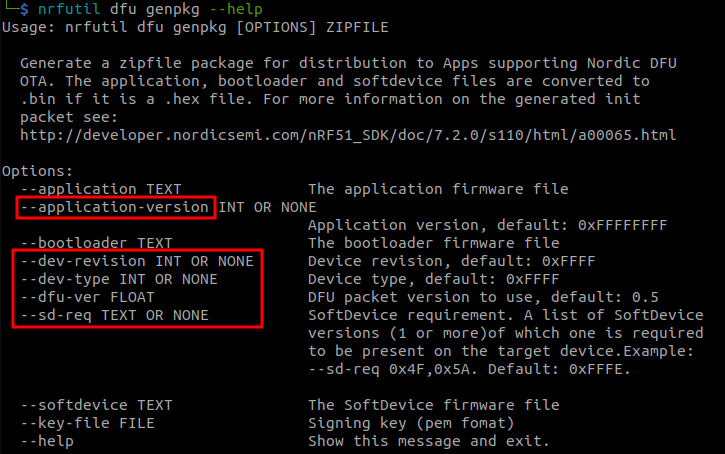
\includegraphics[width=1\linewidth]{../project_Report/images/old-nrfutil-options}
\end{figure}
	
\end{frame}

\begin{frame}
	\frametitle{File .dat}
	dev-type = 3; dev-revision = 4;\\
	application-version = 305441741; sd-req = 0x6789;\\
	0x1234abcd = 305441741; 0x73c6 = 29638; 0x6789 = 26505
	\begin{figure}[H]
		\centering
		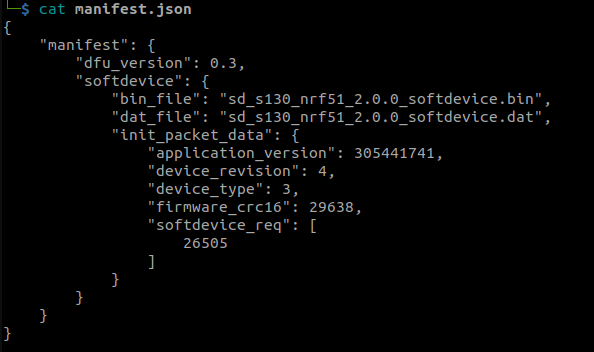
\includegraphics[width=0.7\linewidth]{old-nrfutil-options}
	\end{figure}
	\begin{figure}[H]
		\centering
		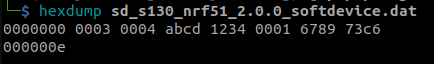
\includegraphics[width=0.7\linewidth]{hexdump-file-dat-open}
	\end{figure}

\end{frame}



	\section{Validation of firmware}
	\subsection{Open bootloader}
	\begin{frame}
		\frametitle{Validation of open bootloader}
		- The information is in available in SDKs
		
		\vspace{0.3cm}
		- The implementation in SDK 11.0.0 includes checks for Device type and revision, Supported SoftDevices, and the checksum, but not for the Application version
		
		\vspace{0.3cm}
		- We can disable the check by not specific it when create
		firmware packages (hence, it will use default values such as 0xFFFF for device type and revision, 0xFFFE for softdevice)
		
		\vspace{0.3cm}
		\pause$\longrightarrow$ No signature\\
		\quad \quad CRC is optional\\
		\quad \quad Validation can be disable by modifying the corresponding value to the default one (we know where is the value)
		
		\vspace{0.3cm}
		\pause$ \longrightarrow $ If an attacker has access to a legitimate firmware, he can craft a bad firmware and pass the firmware validation process
	\end{frame}
	
	\subsection{Secure bootloader}
	\begin{frame}
		\frametitle{Validation of secure bootloader}
		- The information for validation is available in SDKs
		
		\vspace{0.3cm}
		- In brieft, the validation process consists checking some values: Hardware version, SoftDevice version, Firmware version, the hash of the	packet, Signature of the packet, Available space (or Firmware size)\\
		The order of checking may different between SDK versions
		
		\vspace{0.3cm}
		- The acceptance rules for versions
		\begin{itemize}
			\item Hardware version and Softdevice Firmware ID: need to match
			\item Firmware version: $ > $ or $ \geq $
		\end{itemize}

\vspace{0.3cm}
\pause$ \longrightarrow $ If an attacker has access to a good firmware that can do DFU, he/she will know the Hardware and Softdevice of the target\\
+ The tool nrfutil can read the information from a firmware package\\
+ The attacker can also use some tools that can send the init package and wait for responding. The order of checking is different between SDKs, they may be able to distinguish the difference and identify the SDKs version
	\end{frame}

	\section{Summary and Demo}
	\begin{frame}
		\frametitle{Summary}
		\pause- Just by discovering, the attack may identify the type of bootloader: Secure bootloader or open bootloader
		
		\vspace{0.5cm}
		\pause- If the bootloader is open bootloader, the device is vulnerable to Firmware Modification Attack
		
		\vspace{0.5cm}
		\pause- If the firmware is secure bootloader
		
		+ by using signature and CRC, the device may be safe from Firmware Modification Attack\\
		+ by the rules of version acceptance, the device may be safe from Downgrade Attack\\
		+ however, the device can be fingerprinted by the version acceptance rules\\
		+ the order of checking rules is different between SDKs, the attacker may compare the time and fingerprint the device
	\end{frame}
	
	\begin{frame}
		\centering\bf \Huge Demo
	\end{frame}
	
	
	
	\begin{frame}[noframenumbering,plain]
		\centering\bf \Huge Thank you for listening!
	\end{frame}
\end{document}